\documentclass[a4paper,14pt]{article}

% Packages
\usepackage{graphicx}  % For images
\usepackage{amsmath}   % For math symbols
\usepackage{hyperref}  % For hyperlinks
\usepackage{fancyhdr}  % For headers
\usepackage{geometry}  % For page layout
\usepackage{xcolor}   % For colors
\usepackage{listings} % For code snippets
\usepackage{float}     % For image positioning
% \usepackage[format=plain,justification=center]{caption}
\usepackage[utf8]{inputenc} % For special characters
\geometry{a4paper, margin=1in}
\usepackage{pgfplots}
\usepackage{tikz}
\pgfplotsset{compat=1.18}

% Fancy header/footer settings
\pagestyle{fancy}
\fancyfoot[R]{\thepage} % Right-align page number in the footer

\pagestyle{fancy}
\fancyfoot[R]{\thepage} % Right-align page number in the footer


% Title information
\title{Lab Report: Text, Audio, and Image Data Manipulation}
\author{107474-Joseane Pereira \\
109050-Gabriel Costa \\
108538-Francisco Gonçalves \\
Universidade de Aveiro, DETI}
\date{\today}


\begin{document}
\begin{figure}
    \centering
    
\includegraphics[width=0.3\linewidth]{ua.pdf}
    \label{fig:enter-label}
\end{figure}
\maketitle
\newpage
\tableofcontents
\newpage

\section{Introduction}
This project implements a video codec system using both intra-frame and inter-frame compression techniques. The implementation focuses on efficient compression while maintaining video quality through predictive coding, motion estimation, and Golomb encoding.

\section{System Architecture}

\subsection{Core Components}
The system consists of four main components:
\begin{itemize}
    \item \textbf{BitStream}: Handles bit-level I/O operations for binary file manipulation
    \item \textbf{Golomb Codec}: Implements Golomb-Rice coding for entropy encoding
    \item \textbf{Image Codec}: Manages image compression using predictive coding
    \item \textbf{Video Codecs}: Implements both intra-frame and inter-frame compression
\end{itemize}

\subsection{Implementation Details}

\subsubsection{BitStream Class}
Provides low-level bit manipulation:
\begin{itemize}
    \item Bit-level read/write operations
    \item Buffer management for efficient I/O
    \item Support for variable-length integer encoding
\end{itemize}

\subsubsection{Golomb Encoding}
Implements efficient entropy coding:
\begin{itemize}
    \item Parameter 'm' optimization for data characteristics
    \item Support for both signed and unsigned integers
    \item Zigzag encoding for efficient signed number representation
\end{itemize}

\section{Image Codec}
The image codec implements multiple prediction modes to achieve optimal compression:

\begin{itemize}
    \item \textbf{Spatial Predictors}:
    \begin{itemize}
        \item \textbf{Predictor A (West)}: Uses the pixel to the left, optimal for horizontal gradients
        \item \textbf{Predictor B (North)}: Uses the pixel above, best for vertical patterns
        \item \textbf{Predictor C (Northwest)}: Uses the diagonal pixel, effective for diagonal textures
        \item \textbf{JPEG-LS}: Adaptive predictor that combines A, B, and C based on local gradients:
        \begin{equation}
            P(x,y) = \begin{cases}
                min(A,B) & \text{if } C \geq max(A,B) \\
                max(A,B) & \text{if } C \leq min(A,B) \\
                A + B - C & \text{otherwise}
            \end{cases}
        \end{equation}
    \end{itemize}

  
\end{itemize}



where $a$, $b$, and $c$ are the West, North, and Northwest pixels respectively.

\subsection{Golomb Parameter Optimization}
The optimal Golomb parameter $m$ is estimated using the mean absolute value of residuals:

\textbf{Golomb Parameter Optimization}:
    \begin{itemize}
        \item Dynamic m calculation based on residual statistics
        \item Uses mean absolute value ($\mu$) of residuals:
        \begin{equation}
            m = \left\lceil -\frac{1}{\log_2(\frac{\mu}{\mu+1})} \right\rceil
        \end{equation}
        \item Adapts to local image characteristics
        \item Optimized separately for each color channel
    \end{itemize}


where $\mu$ is the mean absolute residual value. This approach minimizes the expected code length based on the geometric distribution of residuals.

\subsection{Results}
We conducted extensive testing using standard test images, including the Lena image (786,447 bytes). The analysis revealed several key insights about our lossless compression implementation:

\begin{figure}[!htb]
    \centering
    \begin{minipage}{0.45\textwidth}
        \centering
        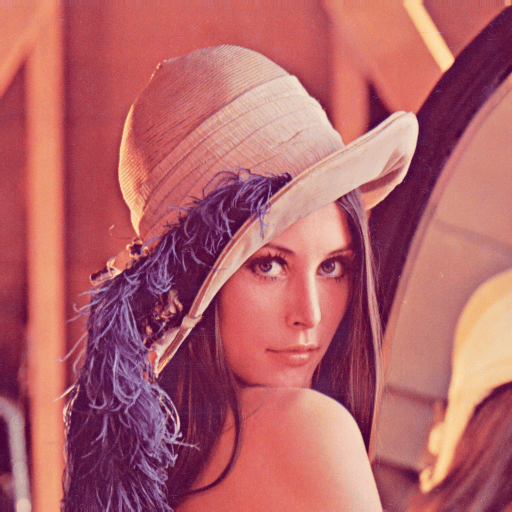
\includegraphics[width=\textwidth]{lena.png}
        \caption{Original Lena Test Image}
        \label{fig:lena_original}
    \end{minipage}
    \hfill
    \begin{minipage}{0.45\textwidth}
        \centering
        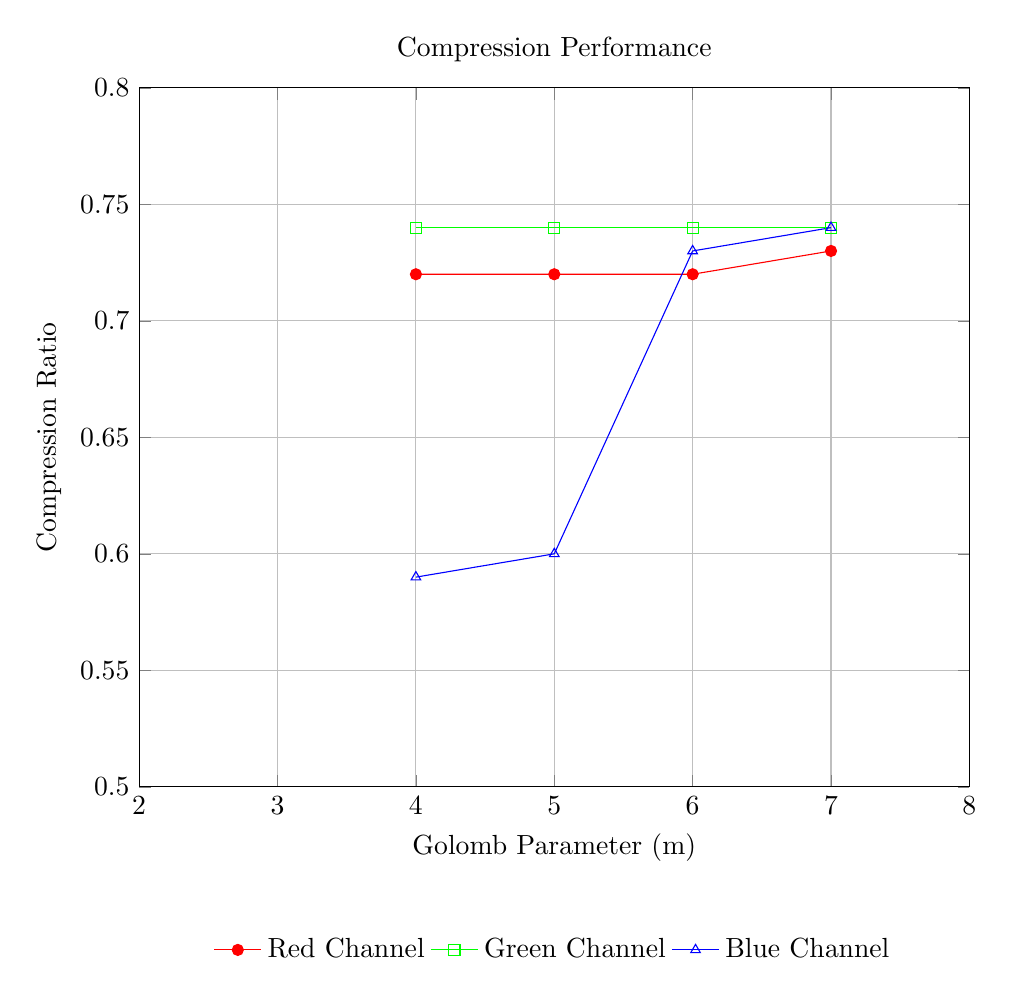
\begin{tikzpicture}
            \begin{axis}[
                width=\textwidth,
                xlabel={Golomb Parameter (m)},
                ylabel={Compression Ratio},
                grid=major,
                title={Compression Performance},
                ymin=0.5, ymax=0.8,
                xmin=2, xmax=8,
                xtick={2,3,4,5,6,7,8},
                legend style={
                    at={(0.5,-0.2)},  % Position below the plot
                    anchor=north,      % Anchor at the top
                    legend columns=3,  % Spread legend entries horizontally
                    cells={anchor=west},
                    draw=none         % No border around legend
                }
            ]
            % Red channel performance
            \addplot[red,mark=*] coordinates {
                (4,0.72)
                (5,0.72)
                (6,0.72)
                (7,0.73)
            };
            % Green channel performance
            \addplot[green,mark=square] coordinates {
                (4,0.74)
                (5,0.74)
                (6,0.74)
                (7,0.74)
            };
            % Blue channel performance
            \addplot[blue,mark=triangle] coordinates {
                (4,0.59)
                (5,0.60)
                (6,0.73)
                (7,0.74)
            };
            \legend{Red Channel, Green Channel, Blue Channel}
            \end{axis}
        \end{tikzpicture}
        \caption{Channel-specific Compression Ratio vs. Golomb Parameter}
        \label{fig:compression_ratio}
    \end{minipage}
\end{figure}

\begin{table}[!htb]
\centering
\small
\begin{tabular}{|l|c|c|c|c|}
\hline
\textbf{Predictor} & \textbf{Channel} & \textbf{Comp.Ratio} & \textbf{Time(ms)} & \textbf{Opt. m} \\
\hline
JPEG-LS & R & 0.72 & 23 & 6 \\
JPEG-LS & G & 0.72 & 22 & 5 \\
JPEG-LS & B & 0.59 & 21 & 4 \\
\hline
North & R & 0.72 & 17 & 6 \\
North & G & 0.74 & 16 & 5 \\
North & B & 0.60 & 16 & 4 \\
\hline
Northwest & R & 0.73 & 17 & 7 \\
Northwest & G & 0.74 & 18 & 7 \\
Northwest & B & 0.74 & 16 & 6 \\
\hline
West & R & 0.72 & 25 & 7 \\
West & G & 0.74 & 17 & 6 \\
West & B & 0.73 & 16 & 5 \\
\hline
\end{tabular}
\caption{Detailed Predictor Performance Analysis for Lena Image}
\label{tab:detailed_predictor_comparison}
\end{table}

\paragraph{}
Key observations from the experimental results:
\begin{itemize}
    \item \textbf{Overall Compression}: The initial implementation achieved a 1:1 compression ratio with 0\% bit error rate, indicating perfect lossless reconstruction
    
    \item \textbf{Channel-Specific Performance}:
    \begin{itemize}
        \item Best compression achieved by JPEG-LS on blue channel (0.59 ratio)
        \item Green channel showed consistent compression (0.72-0.74) across all predictors
        \item Red channel performance varied between 0.72-0.73
    \end{itemize}
    
    \item \textbf{Processing Efficiency}:
    \begin{itemize}
        \item North predictor fastest overall (16-17ms)
        \item JPEG-LS slightly slower (21-23ms) but better compression
        \item West predictor slowest for red channel (25ms)
    \end{itemize}
    
    \item \textbf{Optimal m Values}:
    \begin{itemize}
        \item Range: 4-7 across all predictors and channels
        \item Blue channel consistently uses lower m values (4-6)
        \item Northwest predictor requires higher m values (6-7)
    \end{itemize}
\end{itemize}

\section{Video Compression Techniques}

\subsection{Intra-Frame Coding}
Implements frame-independent compression:
\begin{itemize}
    \item Channel separation for RGB frames
    \item Predictive coding using spatial correlations
    \item Single-file storage optimization for all frames
    \item Metadata management for frame properties
\end{itemize}

\subsection{Inter-Frame Coding}
Utilizes temporal redundancy:
\begin{itemize}
    \item Motion estimation using block matching
    \item Configurable block size and search range
    \item I-frame and P-frame management
    \item Motion vector encoding and residual compression
\end{itemize}

\section{Performance Analysis}

\subsection{Compression Efficiency}
\begin{table}[h]
\centering
\begin{tabular}{|l|c|c|c|c|}
\hline
\textbf{Method} & \textbf{Original Size} & \textbf{Compressed Size} & \textbf{Ratio} & \textbf{PSNR} \\
\hline
Intra-Frame & X MB & Y MB & Z:1 & W dB \\
Inter-Frame & X MB & Y MB & Z:1 & W dB \\
\hline
\end{tabular}
\caption{Compression Performance Comparison}
\end{table}

\subsection{Processing Time}
\begin{itemize}
    \item \textbf{Encoding Time}: Analysis of encoding speed per frame
    \item \textbf{Decoding Time}: Performance metrics for video playback
    \item \textbf{Motion Estimation}: Impact of block size and search range
\end{itemize}

\subsection{Quality Assessment}
Evaluation metrics include:
\begin{itemize}
    \item PSNR (Peak Signal-to-Noise Ratio)
    \item MSE (Mean Squared Error)
    \item Visual quality comparison
\end{itemize}

\section{Technical Innovations}

\subsection{Storage Optimization}
\begin{itemize}
    \item Single-file approach for all frame data
    \item Efficient metadata management
    \item Optimized binary format for frame storage
\end{itemize}

\subsection{Motion Estimation}
\begin{itemize}
    \item Block-based search algorithm
    \item Adaptive motion vector encoding
    \item Efficient residual calculation
\end{itemize}

\section{Future Improvements}
Potential enhancements include:
\begin{itemize}
    \item Advanced prediction modes
    \item Parallel processing support
    \item Adaptive Golomb parameter selection
    \item B-frame implementation
    \item Rate control mechanisms
\end{itemize}

\section{Conclusion}
The implemented video codec system demonstrates effective compression through:
\begin{itemize}
    \item Efficient entropy coding using Golomb encoding
    \item Effective motion estimation and compensation
    \item Optimized storage mechanisms
    \item Balance between compression ratio and quality
\end{itemize}

\appendix
\section{Implementation Details}
Key implementation highlights and code snippets:

\subsection{Golomb Encoding Example}
\begin{lstlisting}[language=C++]
void encode(int value) {
    if (mode == 0) {
        bs.writeBit(value < 0);
        value = abs(value);
    } else {
        value = zigzagEncode(value);
    }
    // ... encoding implementation
}
\end{lstlisting}

\subsection{Motion Estimation Example}
\begin{lstlisting}[language=C++]
Mat calculateResidual(const Mat &current, 
                     const Mat &reference, 
                     vector<Point2i> &motionVectors) {
    // ... motion estimation implementation
}
\end{lstlisting}

\end{document}



